\chapter{AeroShield}

Práca je založená na už započatom projekte vzdušného kyvadla. Na jeho tvorbe sa najviac podieľali študenti: Ján Boldocký, Denis Skokan, Dávid Vereš a Tadeas Vojtko. Prvá verzia dosky a samotného kyvadla, vznikla ako záverečný projekt na predmet Mikropočítače a mikroprocesorová technika. Fotografiu zostavenej dosky, môžeme vidieť na obr.\ref{OBRAZOK 2.1.1}.


\begin{figure}[tbh]
	\centering
	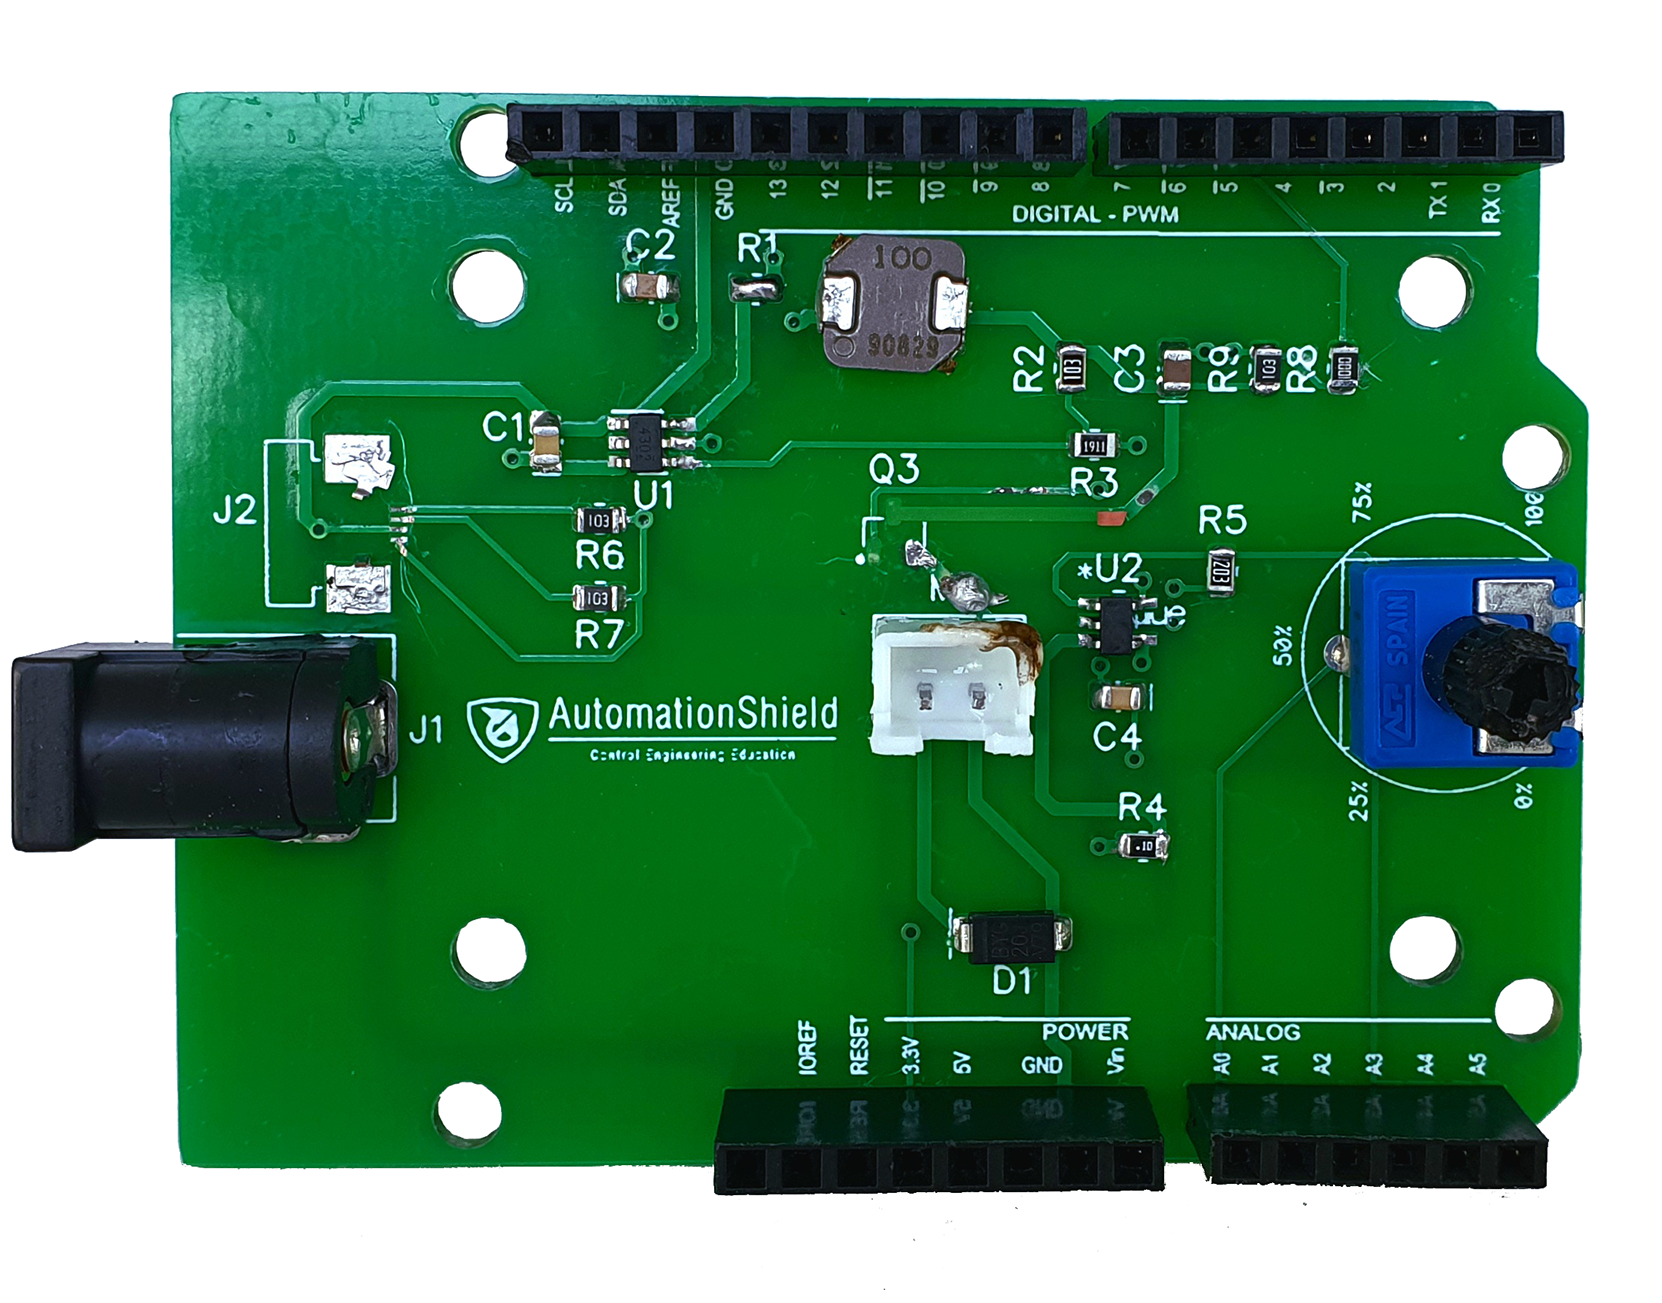
\includegraphics[width=80mm]{obr/oldshield.png}
	\caption{Prvá verzia AeroShieldu.}\label{OBRAZOK 2.1.1}
\end{figure}


V novej verzii dosky bolo odstránených niekoľko nedostatkov predchádzajúcej verzie:

\begin{itemize}
	\item neprepojenie pinov komunikácie I2C tj. piny SDA a SCL senzoru hall efektu, ktorý slúži na meranie uhlu natočenia kyvadla,
	\item nesprávne zapojenie mosfetu PMW45EN, ktorý ovláda PWM signál idúci do akčného člena,
	\item nesprávne umiestnená ochranná dióda na konektoroch akčného člena,
	\item nesprávne zapojený obvod s čipom INA169, ktorý slúži na meranie prúdu,
	\item neprepojenie nulového konektora shieldu s nulovým konektorom arduina.
\end{itemize}

Základom tejto bakalárskej práce teda bolo pochopiť jednotlivé časti zapojenia, ich úprava do funkčnej podoby a následne zostavenie modelu. V rámci projektu bola vytvorená hlavná doska, na ktorej sa nachádza väčšina elektroniky a menšia doska tzv. breakout board obr.\ref{OBRAZOK 2.1.2}.b, ktorý je uchytený v hornej časti kyvadla a slúži na prepojenie senzoru hall efektu s hlavnou doskou shieldu. Doska breakout boardu fungovala bezproblémovo, a teda nebolo potrebné nijakým spôsobom meniť jej schému zapojenia obr.\ref{OBRAZOK 2.1.2}.a. Breakout boardu sa budeme bližšie venovať v časti \ref{PCBcka}.

\begin{figure}[!tbh]
	\hfill
	\subfigure[Schéma zapojenia breakout boardu.]{\includegraphics[width=10cm]{obr/as5600.png}}
	\hfill
	\subfigure[Breakout board.]{\includegraphics[width=5cm]{obr/fotoBreak.png}}
	\hfill
	\caption{Meranie uhla kyvadla.}\label{OBRAZOK 2.1.2}
\end{figure}


\newpage
\section{Hardvér}
\subsection{Popis súčiastok}

V tejto časti sa bližšie pozrieme na menšie celky zapojenia AeroShieldu:
\begin{multicols}{2}
	\begin{itemize}
		\item napájanie,
		\item meranie prúdu,
		\item ovládanie akčného člena,
		\item meranie uhlu kyvadla.
	\end{itemize}
\end{multicols}


\subsubsection{Znižovací menič}
\label{nap}

Na napájanie akčného člena, motorčeka, potrebujeme napätie v rozmedzí 0-3,7 V. Na shield je však privádzané, pomocou koaxiálneho napájacieho konektora, napätie 12 V, ktoré by mohlo motor pri dlhšom používaní zničiť. Na zníženie napätia preto použijeme znižovací menič tzv. buck converter. 

Hlavnou časťou konvertora je čip TPS56339 od výrobcu Texas Instruments obr.\ref{OBRAZOK 2.1}.b. Znižovanie napätia funguje za pomoci dvoch integrovaných N-kanálových 70 m$\Omega$ a 35 m$\Omega$ high-side mosfetov\footnote[4]{N-kanálový mosfet je typ tranzistora, v ktorom sa ovláda kolektorový prúd pomocou napätia medzi riadiacou elektródou a emitorom.}, v spolupráci s ďalšími komponentami. Celkový prevádzkový prúd zariadenia je približne 98 $\upmu$A, keď funguje bez spínania a bez záťaže. Keď je zariadenie vypnuté, napájací prúd je približne 3 $\upmu$A a zariadenie umožňuje nepretržitý výstupný prúd do 3 A\cite{buckobr}.

\begin{figure}[!tbh]
	\hfill
	\subfigure[Schéma zapojenia znižovacieho meniča.]{\includegraphics[width=9cm]{obr/schemaBuck.png}}
	\hfill
	\subfigure[{Čip TPS56339\cite{buckobr}.}]{\includegraphics[width=5cm]{obr/cip.eps}}
	\hfill
	\caption{Znižovací menič.}\label{OBRAZOK 2.1}
\end{figure}

Na čip je privádzané napätie 12 V ktoré sa pomocou zapojenia viditeľného na schéme obr.\ref{OBRAZOK 2.1}.a, znižuje na napätie 3,7 V. Domnievali sme sa, že napájanie motora musí byť realizované externe, pomocou koaxiálneho napájacieho konektora z dôvodu vysokého prúdu odoberaného motorom počas silného zaťaženia. Rovnaký konektor sa síce nachádza aj na doske Arduino UNO a pomocou VIN pinu sa z neho dajú napájať napätím 6-12 V aj iné zariadenia, avšak tento pin je napojený na diódu, obmedzujúcu prúd na 1 A\cite{ampere}\cite{ampere2}. 

Pri testovaní prototypov AeroShieldu, sa merané hodnoty prúdu pohybovali nad hodnotu 1 A, čo by zničilo spomínanú internú diódu na doske Arduino UNO. 
Po zostavení druhej verzie AeroShieldu a opätovnom meraní odoberaného prúdu, bola maximálna dosahovaná hodnota menšia ako 0,5 A. Z tohoto dôvodu sme sa rozhodli pre zmenu v schéme kyvadla, z ktorej sme odobrali externý napájací konektor a následne bola vyrobená nová doska plošných spojov. Tretej verzii AeroShieldu sa bližšie venujeme v časti \ref{tretia}.

\subsubsection{Akčný člen}
\label{akcclen}

Ako akčný člen AeroShieldu je použitý 7 mm, 3,7 V motorček na jednosmerný prúd bez jadra, používaný hlavne pre pohon dronov. “Coreless motor“, alebo motor bez jadra, je motor s cievkou navinutou samou na sebe\cite{coreless}. Stator je vyrobený z magnetov na báze vzácnych zemín, ako je neodým alebo SmCo(samárium-kobalt).

Takýto motor ponúka niekoľko výhod. Výrazne sa znižuje hmotnosť a tým aj zotrvačnosť rotora, čo je dôležité pre naše použitie, kedy potrebujeme dosahovať vysokú akceleráciu motora. Ďalšou výhodou je fakt, že nedochádza k stratám na železe a tým pádom sa účinnosť takýchto motorov blíži až ku 90\%\cite{5545147}. Motor, resp. otáčky motora sú riadené pomocou PWM signálu a ten do motoru prechádza cez N-kanálový mosfet PMV45EN2 od výrobcu Nexperia\cite{pmv}.


\begin{figure}[!tbh]
	\hfill
	\subfigure[Schéma zapojenia motorčeka.]{\includegraphics[width=7cm]{obr/MotorScheme.png}}
	\hfill
	\subfigure[{Akčný člen sústavy.\cite{corelessMotor}}]{\includegraphics[width=7cm]{obr/coreless.jpg}}
	\hfill
	\caption{Zapojenie akčného člena a typ motorčeka.}\label{OBRAZOK 2.3}
\end{figure}


\subsubsection{Meranie prúdu}
\label{merprud}

Z dôvodu merania prúdu odoberaného motorom bol do schémy pridaný monitor prúdu, takzvaný "current shunt monitor". Nameraný prúd môžeme využiť na implementácie riadenia motora na základe prúdu, ktorý odoberá. AeroShield používa snímač INA169NA/250 od výrobcu Texas Instruments obr.\ref{OBRAZOK 2.3.2}.b.

INA169 funguje na základe zaznamenávania zmien napätia na stranách shunt rezistora obr.\ref{OBRAZOK 2.3.2}.a. Na základe nameraného úbytku napätia vysiela senzor podľa nami zvoleného stupňa zosilnenia, napätie s maximálnou hodnotou $V_{OUTMAX} = V_{IN-} - 0.5 V $.

Prúd $I_{s}$ odoberaný motorom, vypočítame pomocou vzorca \ref{Shunt}

\begin{align}
	\label{Shunt}
 I_{s} = \dfrac{(V_{OUT} \times  1 k\Omega)}{(R_{s} \times R_{l})}
\end{align}

kde $V_{OUT}$ je napätie namerané na výstupe, 1 k$\Omega$ je konštanta vnútorných odporov senzoru, $R_{s}$ je hodnota bočníka v $\Omega$ a $R_{l}$ je hodnota rezistora na výstupe, taktiež v $\Omega$\cite{INA}.

\begin{figure}[!tbh]
	\hfill
	\subfigure[Schéma zapojenia snímača prúdu.]{\includegraphics[width=9cm]{obr/INAschema.png}}
	\hfill
	\subfigure[{Senzor INA169NA/250\cite{INAobr}.}]{\includegraphics[width=6cm]{obr/ina.png}}
	\hfill
	\caption{Meranie prúdu.}\label{OBRAZOK 2.3.2}
\end{figure}


\subsubsection{Meranie uhla kyvadla}
\label{meruhl}

Na fungovanie AeroShieldu je dôležité vedieť s vysokou presnosťou merať uhol naklonenia kyvadla. Na tento účel sme si zvolili meranie uhlu bezkontaktnou formou, pomocou snímača Hallovho javu. Hallov jav vieme opísať ako vznik priečneho elektrického poľa v pevnom materiáli, keď ním preteká elektrický prúd a tento materiál je umiestnený v magnetickom poli, ktoré je kolmé na prúd\cite{Hall}. Toto elektrické pole, resp. vznik elektrického potenciálu, vieme detegovať ako Hallovo napätie a na základe jeho zmeny, vieme určiť rotáciu kyvadla. Fyzikálna podstata tohoto javu je na obr.\ref{OBRAZOK 1.323}, kde V$_H$(V) je Hallovo napätie, B(T) je magnetické pole, F$_m$(N) magnetická sila pôsobiaca na negatívne prenášače náboja, F$_e$(C) elektrická sila z nahromadeného náboja, I(A) je dohodnutý smer elektrického prúdu. 

\begin{figure}[!tbh]
	\centering
	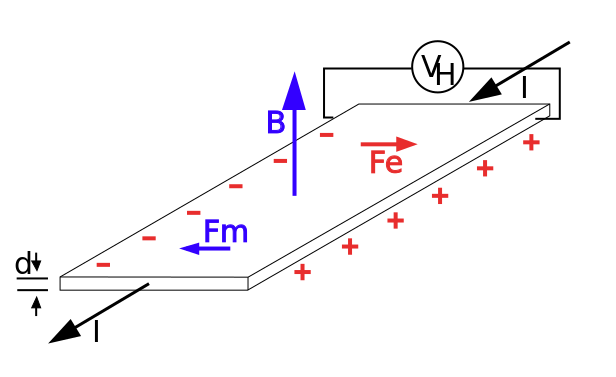
\includegraphics[width=100mm]{obr/hallovjav.png}
	\caption{Schematická reprezentácia hallovho javu.}\label{OBRAZOK 1.323}
\end{figure}

V kyvadle je na konci horizontálneho ramena umiestnený špeciálny magnet kruhového tvaru, ktorý je polarizovaný naprieč prierezom magnetu. Ako senzor na meranie hall efektu je použitý AS5600 od výrobcu OSRAM obr.\ref{OBRAZOK 2.2}.b. Signály zachytené senzorom sa v čipe najskôr zosilnia, následne sú filtrované a prechádzajú konverziou pomocou analógovo-digitálneho prevodníka(ADC). Snímaná je aj intenzita magnetického poľa, ktorou senzor pomocou
automatického riadenia zosilnenia(AGC) kompenzuje zmeny teploty priestoru a taktiež zmeny sily magnetického poľa.

Na výber sú dva typy výstupu a to analógový, alebo digitálny výstup s kódovaním PWM. Senzor má taktiež možnosti interného programovania pomocou rozhrania I2C.
V našom prípade používame 12-bitový analógový výstup s rozlíšením 0°5'16". Toto rozlíšenie nám umožňuje s vysokou presnosťou kontrolovať naklonenie kyvadla a na základe získaných informácii ovplyvňovať fungovanie akčného člena sústavy. Schéma zapojenia enkóderu na meranie uhla môžeme vidieť na obr.\ref{OBRAZOK 2.2}.a.



\begin{figure}[!tbh]
	\hfill
	\subfigure[Schéma zapojenia čipu AS5600.]{\includegraphics[width=10cm]{obr/as5600.png}}
	\hfill
	\subfigure[{Čip AS5600\cite{As5600obr}.}]{\includegraphics[width=4cm]{obr/hall.jpg}}
	\hfill
	\caption{Enkóder slúžiaci na meranie uhla kyvadla.}\label{OBRAZOK 2.2}
\end{figure}

\newpage


\subsection{Schéma zapojenia}

Všetky schémy zapojenia boli tvorené v bezplatnej verzii programu DipTrace, ktorý slúži ako prostredie na tvorbu elektrotechnických schém a dosiek plošných spojov. 

Nie všetky komponenty potrebné na tvorbu schémy zapojenia boli zahrnuté v knižniciach DipTracu, avšak tieto komponenty sú dostupné na stránkach výrobcov, odkiaľ sa dajú stiahnuť a následne použiť v schéme\cite{AS5600Downl}\cite{TPS56339Downl}\cite{INAobr}. Do programu bola taktiež vložená knižnica AutomationShieldu, ktorá obsahuje najčastejšie používané komponenty. Jednotlivé komponenty majú podobu elektrotechnických značiek s danými vlastnosťami. 

Polohu volíme takú, aby schéma bola čo najprehľadnejšia a komponenty, ktoré sú medzi sebou prepojené, boli čo najbližšie pri sebe. Akonáhle máme všetky komponenty uložené začneme s ich postupným prepájaním. Pri zapájaní jednotlivých komponentov sa riadime ich priloženými katalógovými listami, v ktorých býva častokrát aj návrh schémy zapojenia a spôsobu využitia daného komponentu.

DipTrace umožňuje rozdielne zafarbovanie jednotlivých elektrických spojení, rozličnými farbami a názvami obr.\ref{OBRAZOK 2.3.5}. Tento fakt nám veľmi uľahčuje, na prvý pohľad rozoznať napríklad elektrické zemniace spojenie- zelená, fázové spojenia 3,3V- červená. Na schéme zapojenia sú použité nasledujúce komponenty:
\begin{multicols}{3}
	\begin{itemize}
		\item R- Rezistor
		\item C- Kapacitor
		\item J- Konektor
		\item U- Mikročip
		\item L- Cievka
		\item D- Dióda
		\item M- Motor
	\end{itemize}
\end{multicols}


\begin{figure}[!tbh]
	\includegraphics[width=\textwidth]{obr/aeroSchema.png}
	\caption{Schéma zapojenia AeroShieldu.}\label{OBRAZOK 2.3.5}
\end{figure}

\subsection{Doska plošných spojov}
\label{PCBcka}

Po návrhu a kontrole schém zapojenia sa schémy ďalej spracovávajú do podoby dosky plošných spojov. Schémy exportujeme do programu DipTrace PCB v ktorom máme následne niekoľko možností postupu. Jednotlivé komponenty sa nám už zobrazujú v reálnej podobe, takže vidíme ich veľkosť a rozmiestnenie konektorov na spájkovanie. Dosky plošných spojov majú niekoľko výhod, ale aj negatív oproti ponúkaným alternatívam\cite{dosky}. 

Výhodou je fakt, že vodivé spojenia medzi jednotlivými súčiastkami sú narozdiel od typických káblových spojení, realizované vrstvou medi, ktorá je ukrytá pod ochrannými vrstvami dosky. Ďalšou z výhod dosiek plošných spojov je skutočnosť, že sú odolné a kompaktné\cite{PCBlife}. Tým že vodivé cesty môžu mať veľmi malé rozmery, ovplyvňujúcim faktorom veľkosti dosky plošných spojov je samotná veľkosť použitých komponentov. 

Nevýhodami sú napríklad vyššia cena, ako pri spojení pomocou káblov, zložitý proces výroby, ktorý predlžuje čakaciu dobu na hotový produkt. Ďalšou z nevýhod je zložitá, alebo nemožná oprava chyby na hotovej doske, ktorá nastala v procese tvorby schémy zapojenia . 

Hotová schéma zapojenia je prenesená do programu DipTrace PCB. Program ponúka možnosť automatického alebo manuálneho rozmiestnenia komponentov.

\begin{figure}[!tbh]
	\hfill
	\subfigure[Vrchná strana breakout boardu.]{\includegraphics[width=5cm]{obr/breakoutTOP.png}}
	\hfill
	\subfigure[Spodná strana breakout boardu.]{\includegraphics[width=5cm]{obr/breakoutbottom.png}}
	\hfill
	\caption{Breakout board.}\label{OBRAZOK 2.6}
\end{figure}

Po rozmiestnení komponentov treba jednotlivé piny poprepájať vodivými cestami, ktoré nahrádzajú funkciu káblov. Máme možnosť zvoliť automatické alebo manuálne rozmiestnenie ciest. Ako je vidieť na obr.\ref{OBRAZOK 2.4}.a, nie všetky cesty majú rovnakú šírku. Dôvodom je fakt, že niektorými cestami prúdi väčší prúd. V zásade sa používa pravidlo, čím vyšší prúd preteká vodičom, tým väčšiu plochu prierezu by mal mať. Prúdy pretekajúci vodičom tento vodič zahrieva. Pokiaľ je toto zahrievanie nadmerné, môže dôjsť k poškodeniu vodiča.  

Tvorba elektrických ciest má niekoľko pravidiel. Najdôležitejšie z nich je, že cesty spájajúce rozdielne vodiče sa nemôžu križovať. Pokiaľ by k takémuto kríženiu došlo, jednotlivé cesty sa vzájomne vyskratujú. Z toho dôvodu treba niekedy cestu priviesť na druhú stranu dosky plošných spojov, kde v jej pokračovaní neprekáža iná cesta. Na tento účel sa používajú vodivé konektory ,,via'', spájajúce obe strany dosky. Tretia verzia dosky AeroShieldu je na obr.\ref{OBRAZOK 2.4}. 

Po finálnej kontrole zapojenia komponentov na doske plošných spojov môžeme tieto dosky uložiť do formátu gerber. Súbory typu gerber v sebe ukladajú presné zloženie finálnej dosky plošných spojov a to po jej jednotlivých vrstvách. Zkonvertované súbory zasielame výrobcovi PCB dosiek, kde si môžeme zvoliť parametre dosky ako jej farbu, typy spájkovacích doštičiek a iné. Podobu finálnej dosky AeroShieldu môžeme vidieť na obr.\ref{OBRAZOK 2.7}.a a dosky breakout boardu na obr.\ref{OBRAZOK 2.7}.b.

\begin{figure}[!tbh]
	\centering
	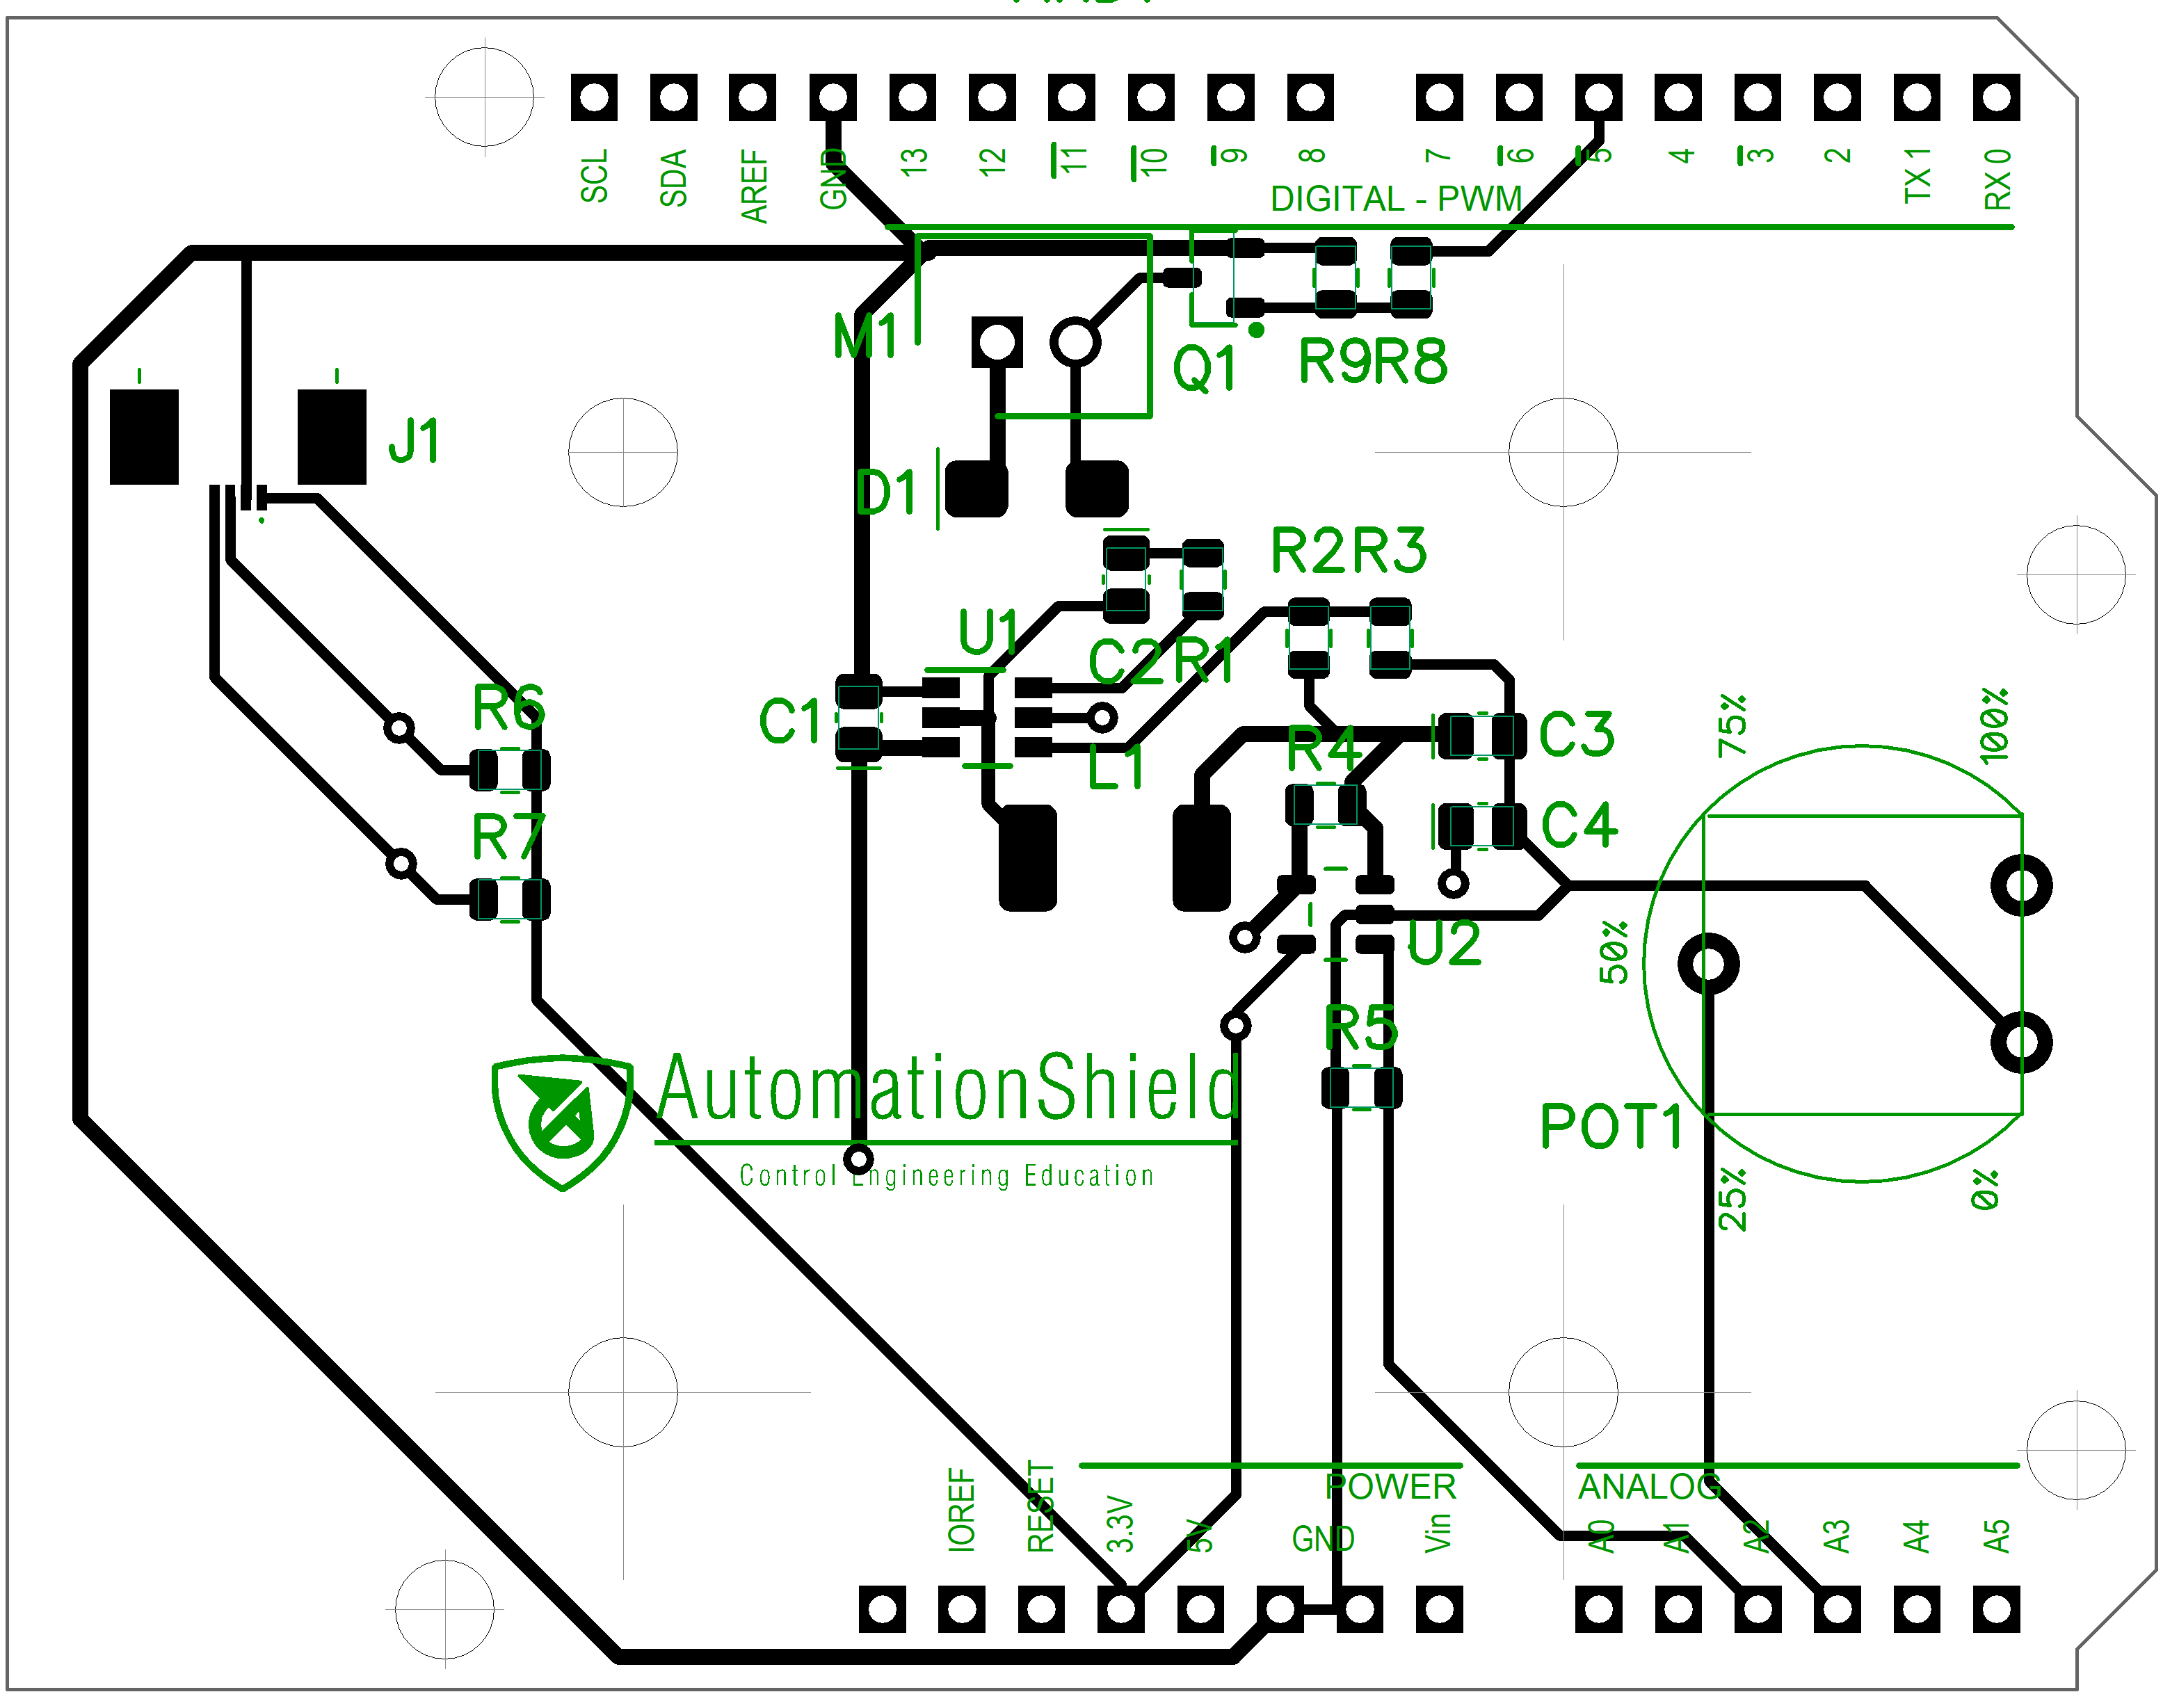
\includegraphics[width=8cm]{obr/AeroShield3TOP.png}
	
	(a)
	
	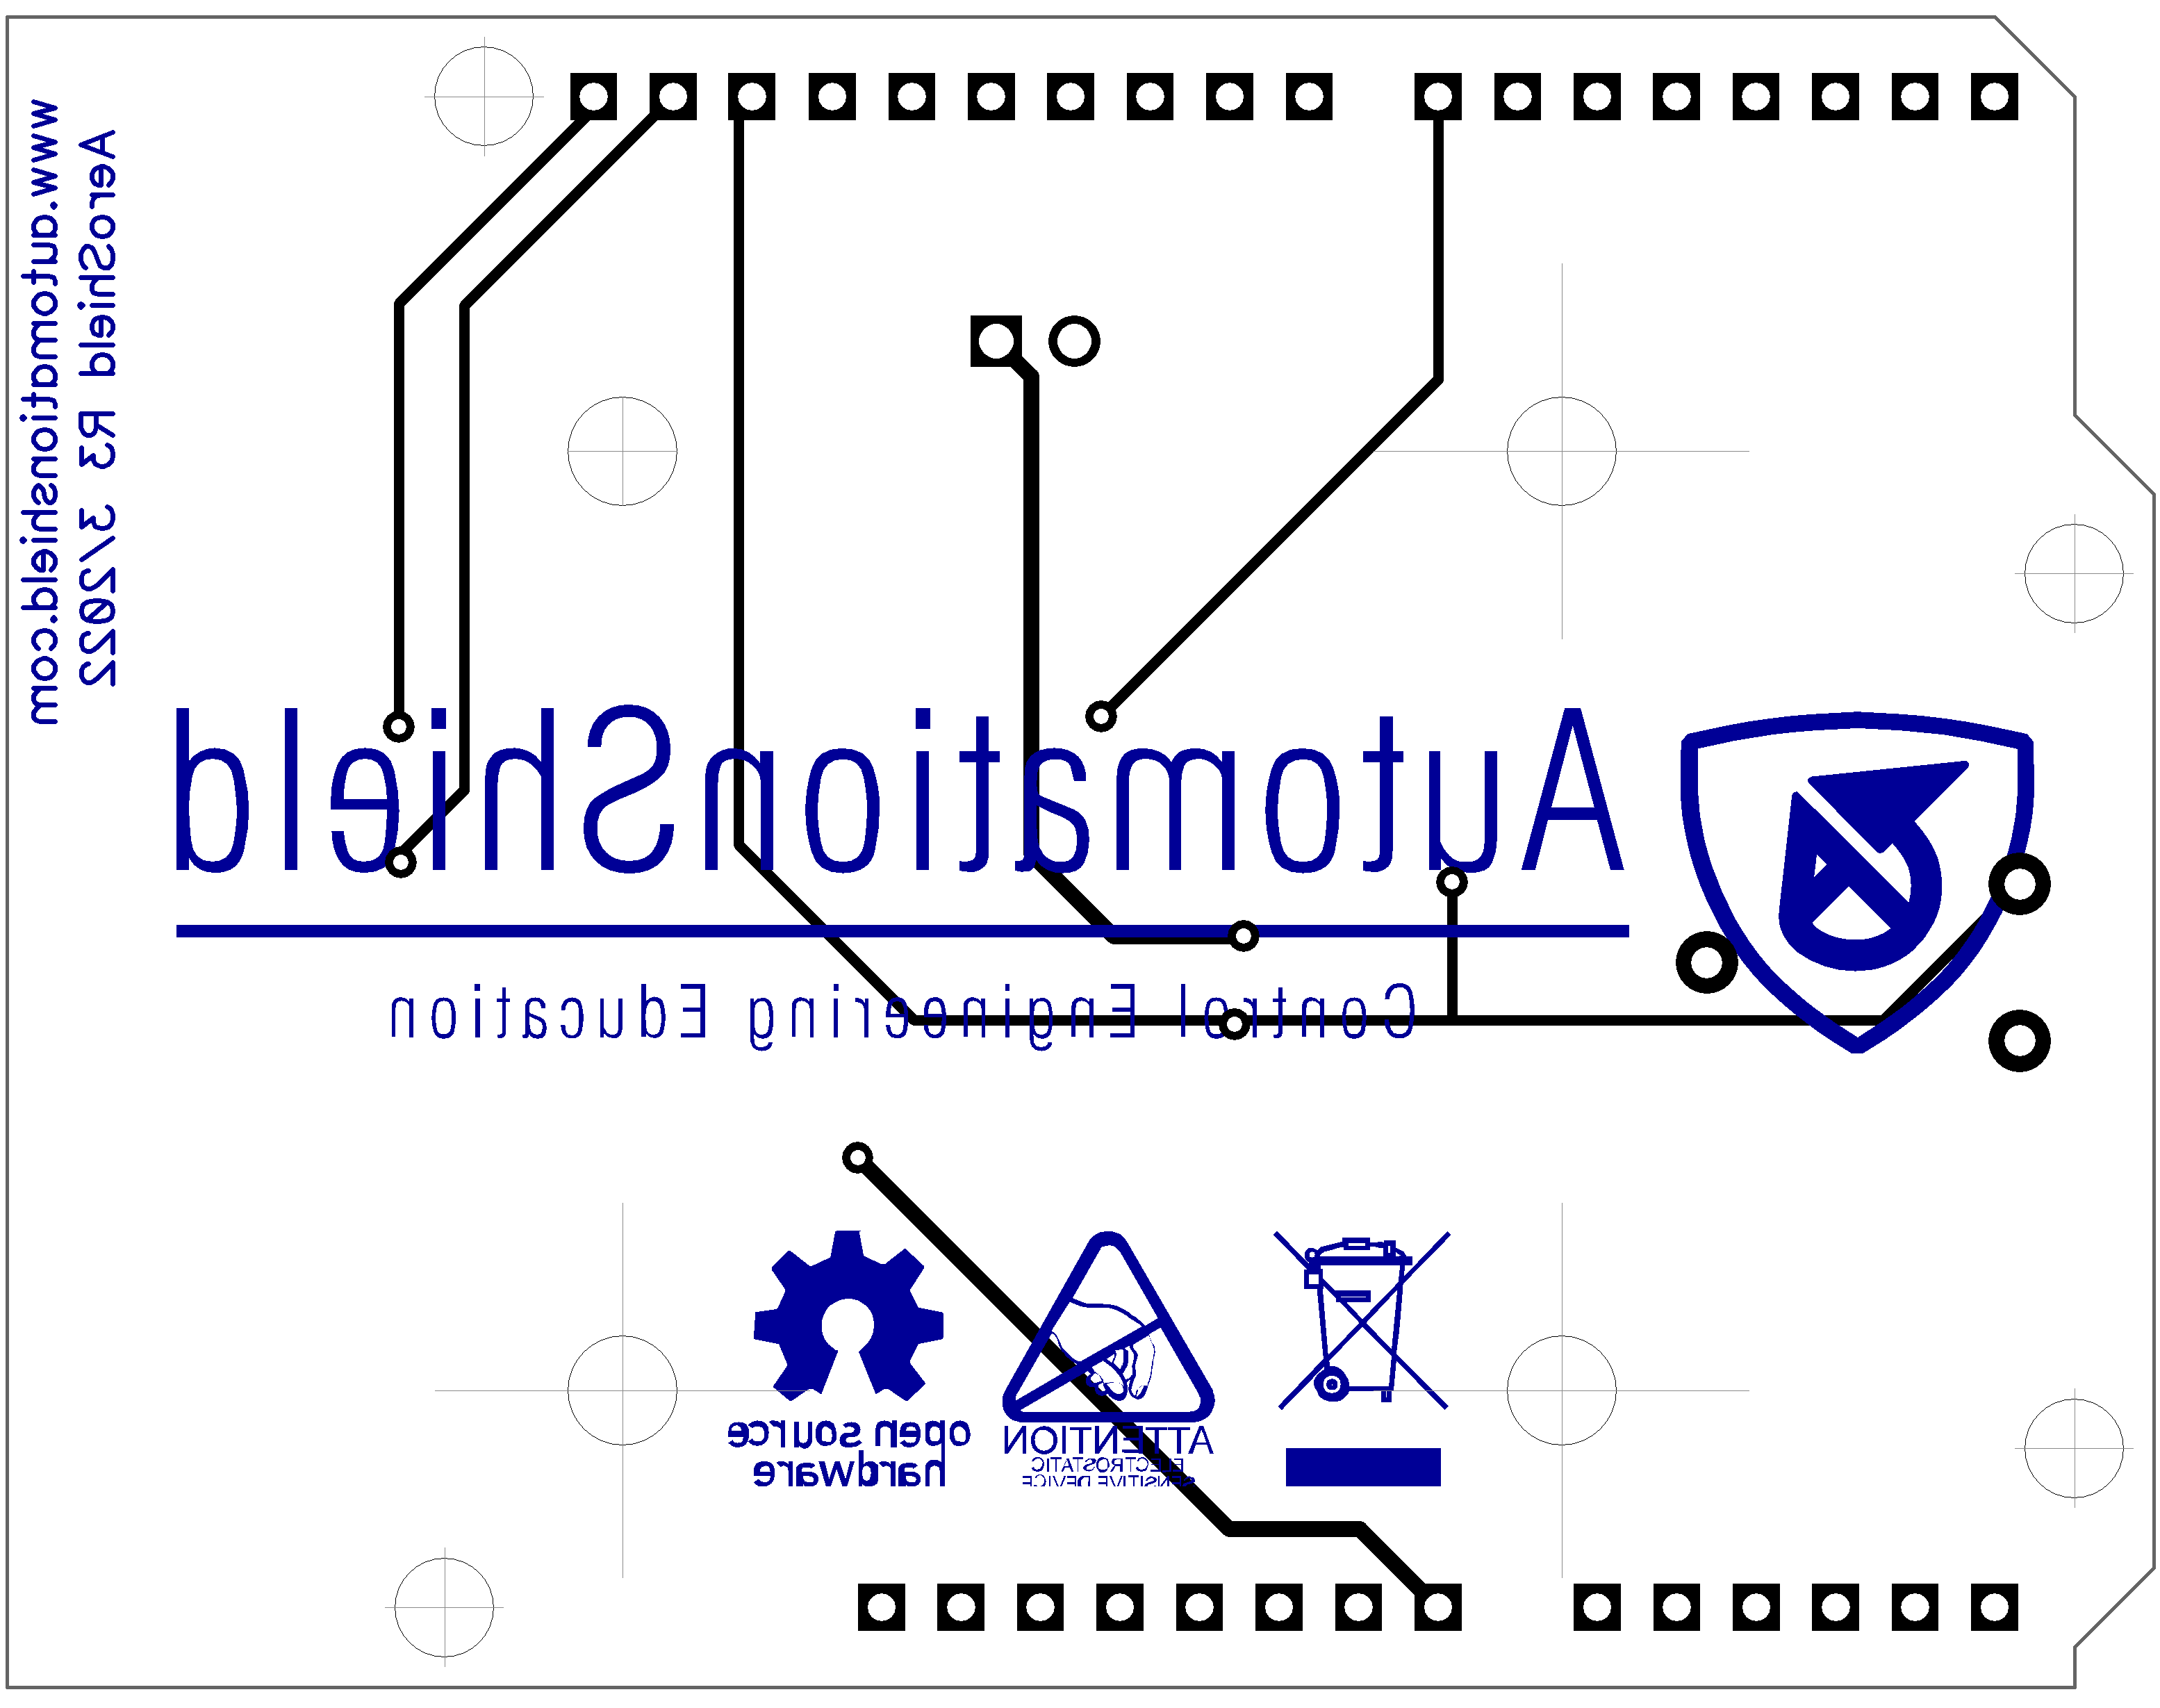
\includegraphics[width=8.5cm]{obr/AeroShield3BOTTOM.png}
	
	(b)
	
	\caption{(a) Vrchná strana AeroShieldu. (b) Spodná strana AeroShieldu.}
	\label{OBRAZOK 2.4}
\end{figure}



\begin{figure}
	\hfill
	\subfigure[Hlavná doska AeroShieldu.]{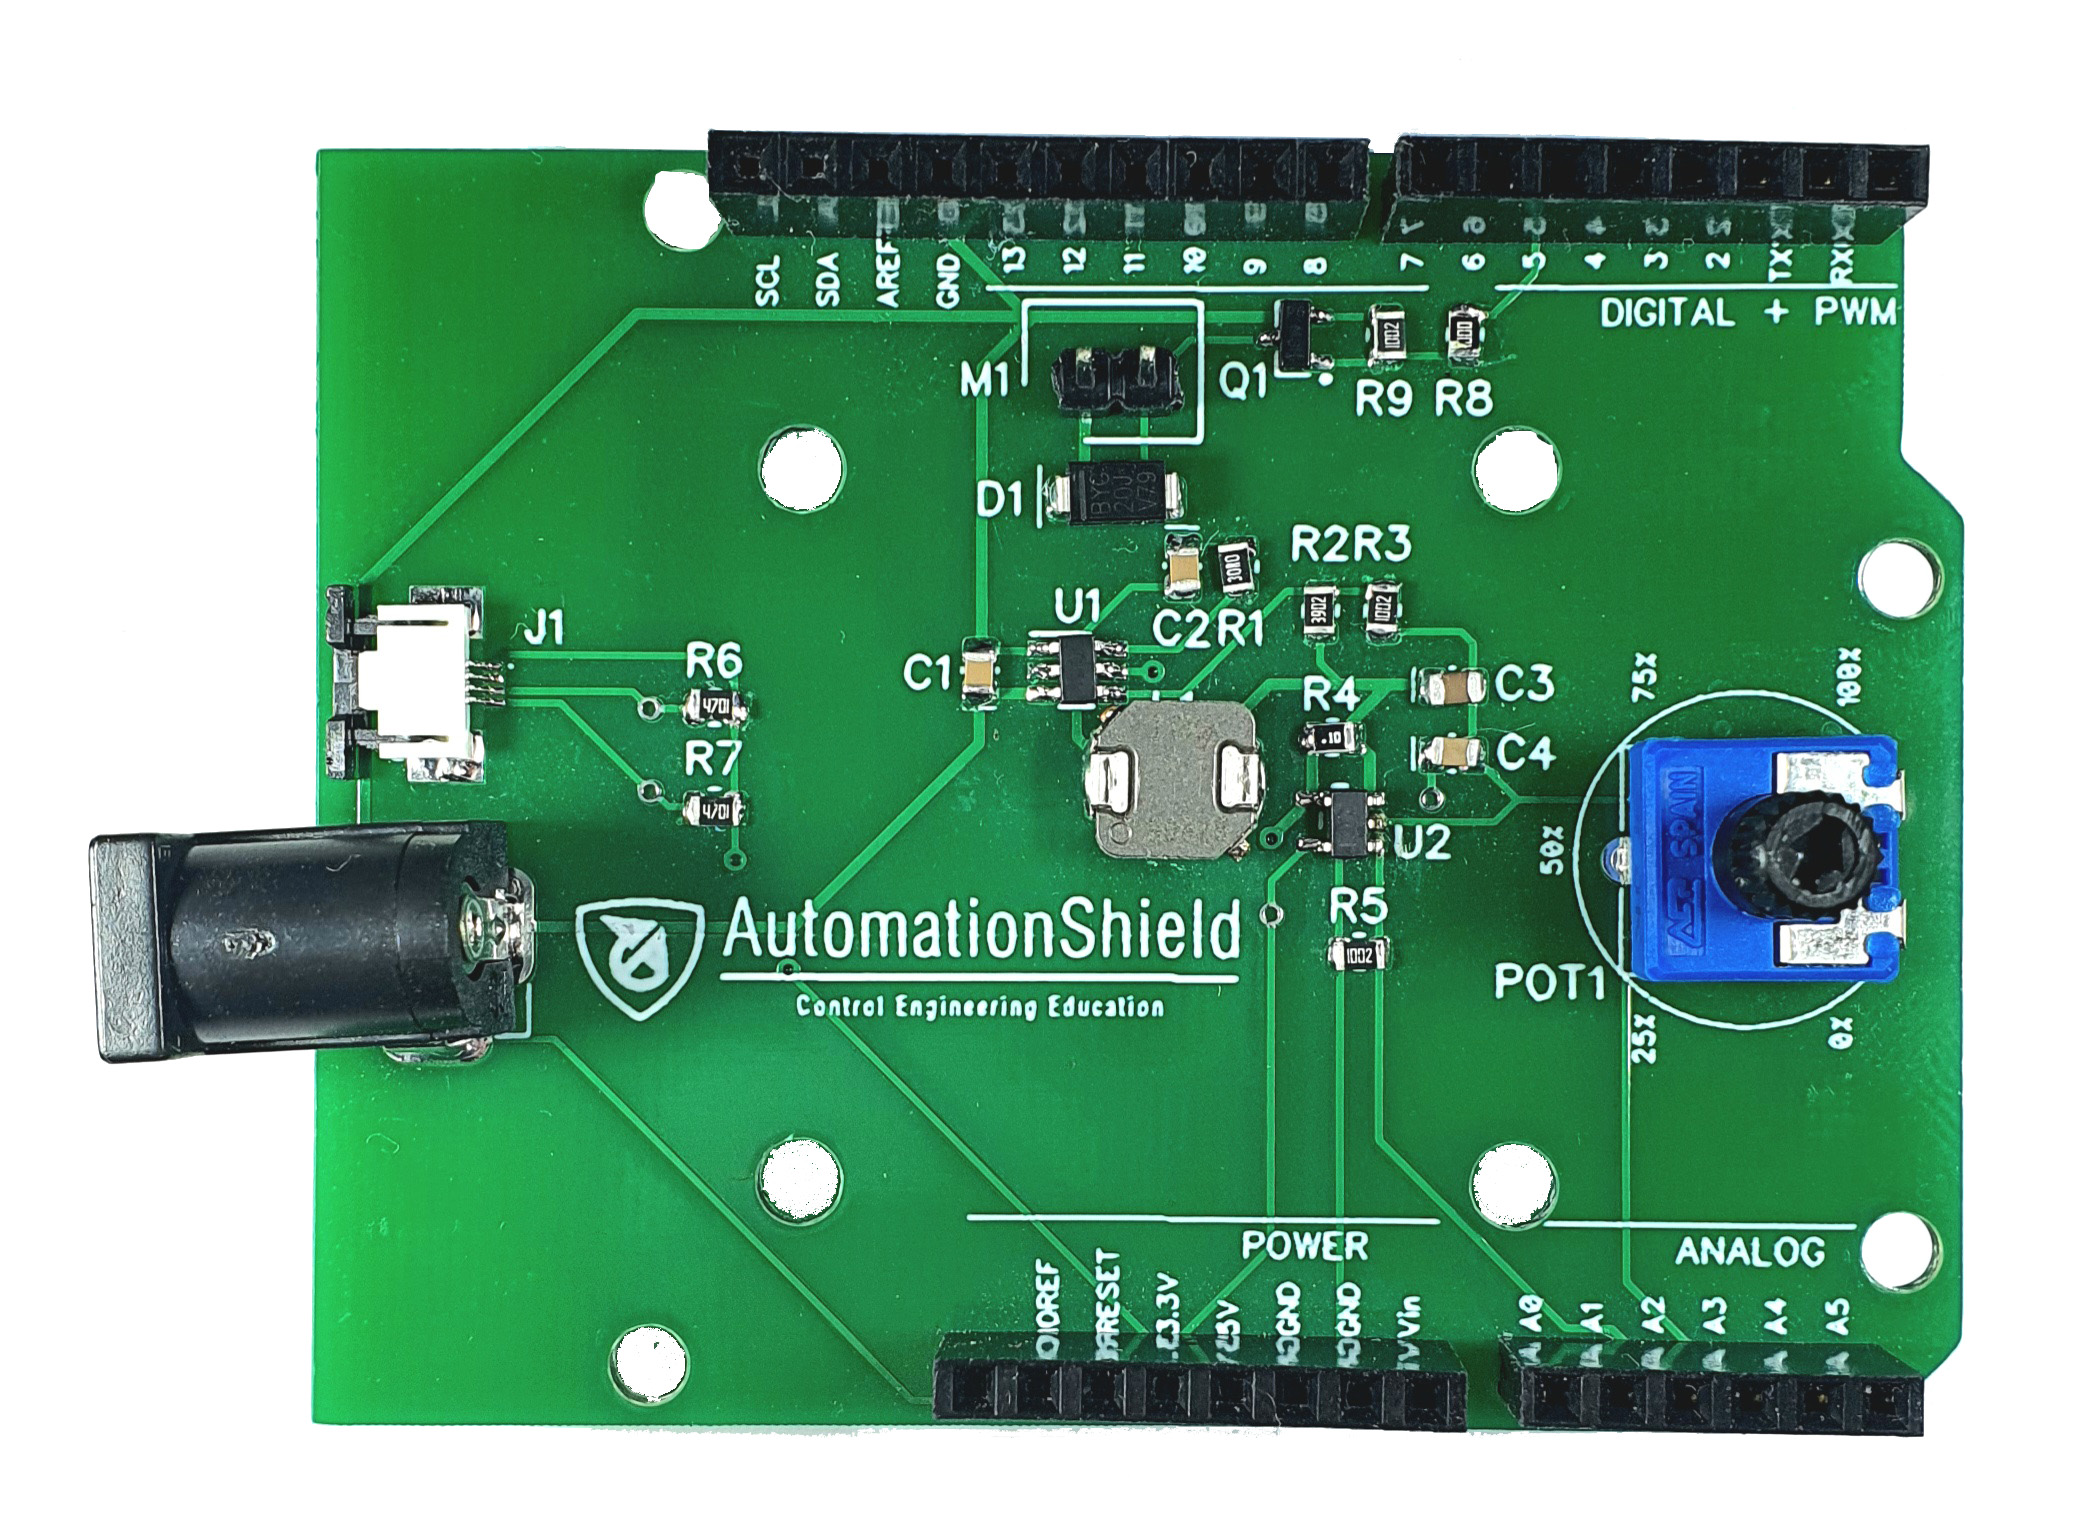
\includegraphics[width=9cm]{obr/AeroShield.jpg}}
	\hfill
	\subfigure[Vedľajšia doska AeroShieldu.]{\includegraphics[width=6cm]{obr/fotoBreak.png}}
	\hfill
	\caption{Dosky plošných spojov AeroShieldu (2. verzia).}\label{OBRAZOK 2.7}
\end{figure}

\subsection{Model držiaku kyvadla}
\label{telo}

Telo kyvadla ako aj všetky konektory spájajúce jeho jednotlivé časti, boli vytvorené v 3D modelovacom softvéri CATIA obr.\ref{OBRAZOK 1.1}. Zámerom bolo vytvoriť pevný a zároveň estetický držiak, ktorý sa dá následne vytlačiť na 3D tlačiarni. Telo kyvadla stojí na štyroch nožičkách, ktoré sú priskrutkované k hlavnej doske plošných spojov. Stred kyvadla je dutý, a sú nim vedené káble napájania motorčeka. V hornej časti držiaku sa nachádzajú diery na priskrutkovanie breakout boardu. 

\begin{figure}
	\hfill
	\subfigure[Model tvorený v programe CATIA.]{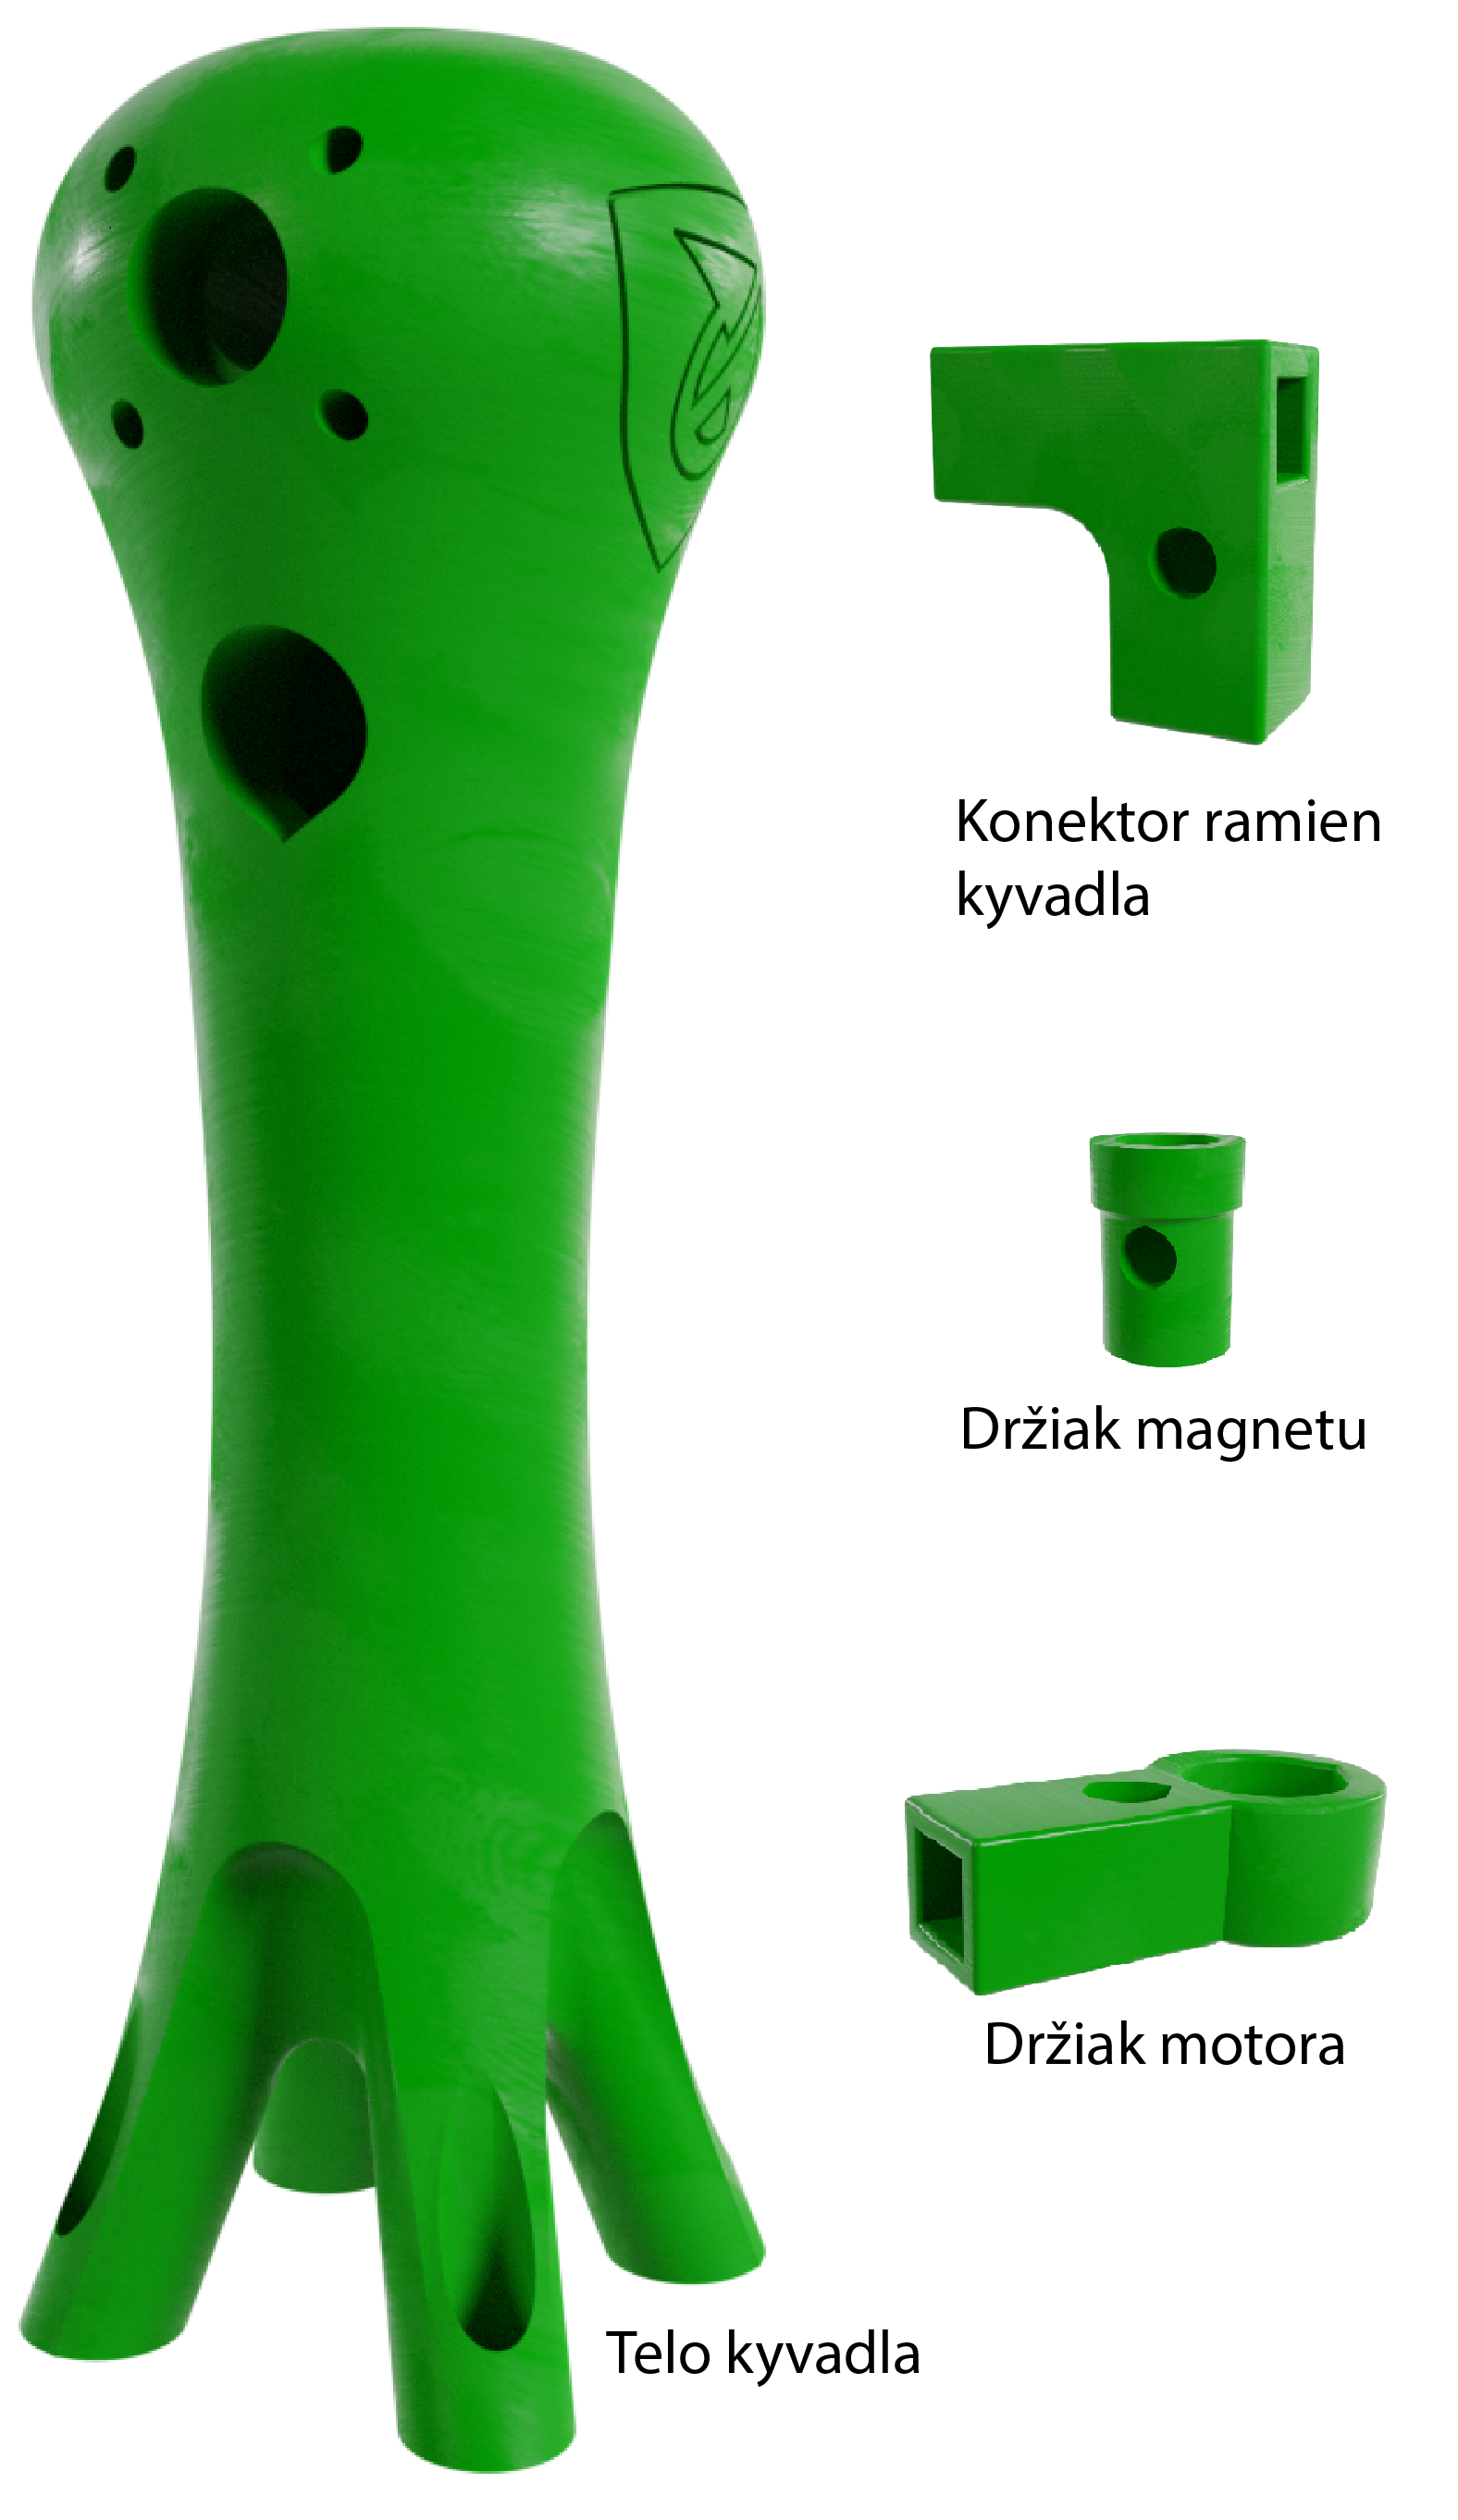
\includegraphics[width=65mm]{obr/spojeneKyvadlo.png}}
	\hfill
	\subfigure[Zostavený model AeroShieldu.]{\includegraphics[width=58mm]{obr/BezPozadnia.png}}
	\hfill
	\caption{AeroShield.}\label{OBRAZOK 1.1}
\end{figure}


\subsubsection{Cenová kalkulácia AeroShieldu}

Hlavnou podmienku pri tvorbe AeroShieldu bola jeho funkcionalita, dostupnosť použitých komponentov, jednoduchosť vyhotovenia, ako aj nízka cena zostaveného modelu. Za účelom predstavy cenovej jedného kusu AeroShieldu, bola zostavená tabuľka\ref{Cenova kalkulacia} s použitými komponentami, ich počtom a reálnou kúpnou cenou v eurách(spolu s DPH). Pri komponentoch ako sú rezistory a kapacitory, bola cena určená ako priemerná hodnota týchto komponentov pri kúpe viac ako 100kusov, keďže pri kúpe zopár kusov(1-20) je ich cena rádovo vyššia, ako cena pri nákupoch viacero kusov. 

\begin{table}
	\begin{tabular}{p{0.25\textwidth} p{0.43\textwidth} p{0.05\textwidth} p{0.07\textwidth} p{0.07\textwidth}}
		\hline
		\multicolumn{1}{|l}{\textbf{Názov}} & \textbf{Popis}                                     & \multicolumn{1}{l}{\textbf{Ks.}} & \multicolumn{1}{l}{\textbf{Cena v \euro}} & \multicolumn{1}{l|}{\textbf{Spolu}} \\ \hline
		Kapacitor                           & SMD, sot23                                         & 6                                  & 0,08                                      & 0,48                                        \\
		Dióda                               & 1N400IG                                            & 1                                  & 0,1                                      & 0,1                                        \\
		FFC konektor                        & FFC 4pin                                           & 2                                  & 0,2                                      & 0,4                                        \\
		Cievka                              & IND1210                                            & 1                                  & 0,2                                      & 0,2                                        \\
		Konektor DC motora                  & JST-XH 2,54                                        & 1                                  & 0,4                                      & 0,4                                        \\
		Motor                               & Howellp 7x20 mm Motor                               & 1                                  & 2,1                                      & 2,1                                        \\
		Potenciometer                       & CA14                                               & 1                                  & 0,45                                     & 0,45                                       \\
		Mosfet                              & pmv45en2                                           & 1                                  & 0,04                                     & 0,04                                       \\
		Rezistor                            & SMD, sot23                                         & 9                                  & 0,08                                      & 0,72                                        \\
		Buck converter                      & TPS56339                                           & 1                                  & 2,78                                     & 2,78                                       \\
		Shunt monitor                       & INA169/NA                                          & 1                                  & 0,98                                     & 0,98                                       \\
		Hall senzor                         & AS5600                                             & 1                                  & 1,48                                     & 1,48                                       \\
		3D komponenty                       & model kyvadla a spojovacie prvky                   & 4                                  & 2,2                                      & 2,2                                        \\
		Gulôčkové ložiská                   & BB-694-B180-30-ES IGUS                             & 2                                  & 2,75                                     & 5,5                                        \\
		Prepájacie káble FFC                & akékoľvek 4 pin, dĺžka min 15cm                    & 1                                  & 0,52                                     & 0,52                                       \\
		Prepajací kábel motor               & akékoľvek, dĺžka min 35cm                          & 1                                  & 0,3                                      & 0,3                                        \\
		Šróby                               & 4x M3x40 4x M4x15                                  & 8                                  & 0,25                                     & 2                                          \\
		Karbónové trubičky                  & 1x kruhový prierez 10cm, 1x štvorcový prierez 10cm & 2                                  & 1,9                                      & 3,8                                        \\
		PCB shield                          & Výroba JLCPCB                                      & 1                                  & 0,35                                     & 0,35                                       \\
		PCB brakout                         & Výroba JLCPCB                                      & 1                                  & 0,35                                     & 0,35                                       \\
		Matice                              & M4                                                 & 4                                  & 0,2                                      & 0,8                                        \\ \hline
		\multicolumn{1}{|l}{}               &                                                    & \multicolumn{1}{l}{}               & \textbf{Spolu}                           & \multicolumn{1}{c|}{\textbf{25,95\euro}}        \\ \hline
	\end{tabular}
\caption{Cenová kalkulácia AeroShieldu.}
\label{Cenova kalkulacia}
\end{table}

\subsection{Tretia verzia AeroShieldu}
\label{tretia}

V tretej verzii AeroShieldu obr.\ref{OBRAZOK 2.8}, bol odstránený napájací konektor a napájanie je realizované z konektora, ktorý sa nachádza na doske Arduino. Na Shield je napätie 12V privádzané pomocou \verb|vin| pinu obr.\ref{OBRAZOK 2.9}. Prúd odoberaný motorom nedosahuje hodnoty väčšie ako 1A a teda takéto napájanie je bezpečné a nehrozí pri ňom poškodenie hardvéru Arduina. Ďalej bolo upravené rozloženie niektorých komponentov. Jedná sa hlavne o konektor \verb|J1|, spájajúci hlavnú dosku s breakout doskou, rezistory \verb|R8, R9| a mosfet \verb|Q1|. Ako posledná úprava bola otočená polarita potenciometra, ktorý bol na druhej verzii AeroShieldu pripojený opačne, ako značil popis na doske. 

\begin{figure}[!tbh]
	\centering
	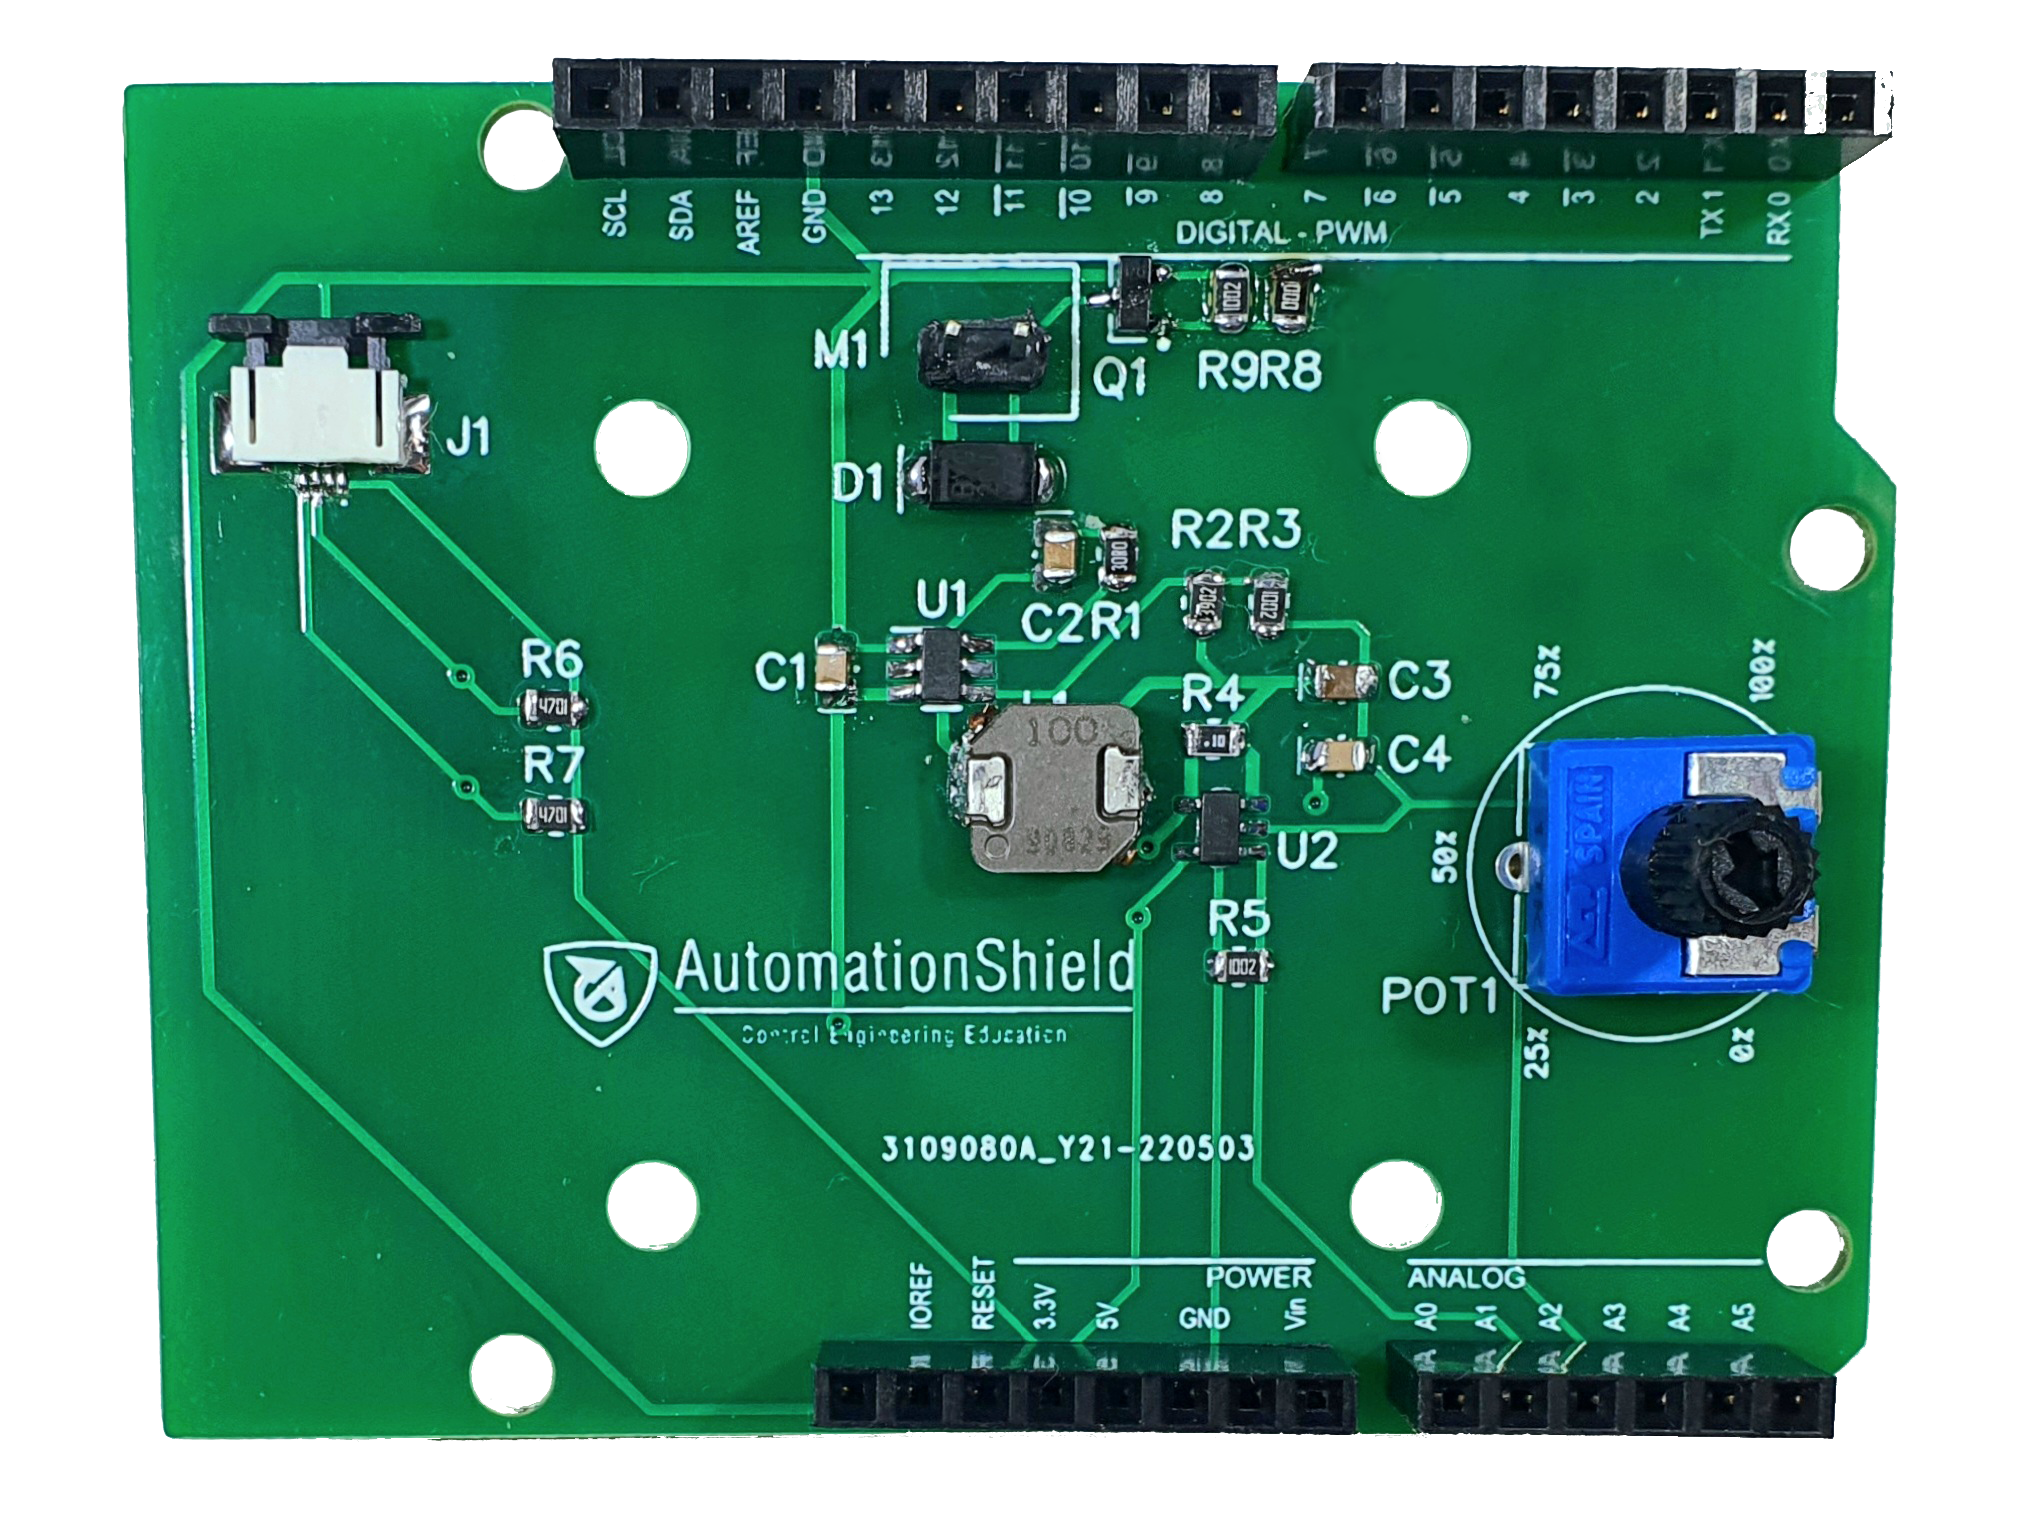
\includegraphics[width=110mm]{obr/NewAeroShield.png}
	\caption{Tretia verzia AeroShieldu.}\label{OBRAZOK 2.8}
\end{figure}

\begin{figure}[!tbh]
		\centering
	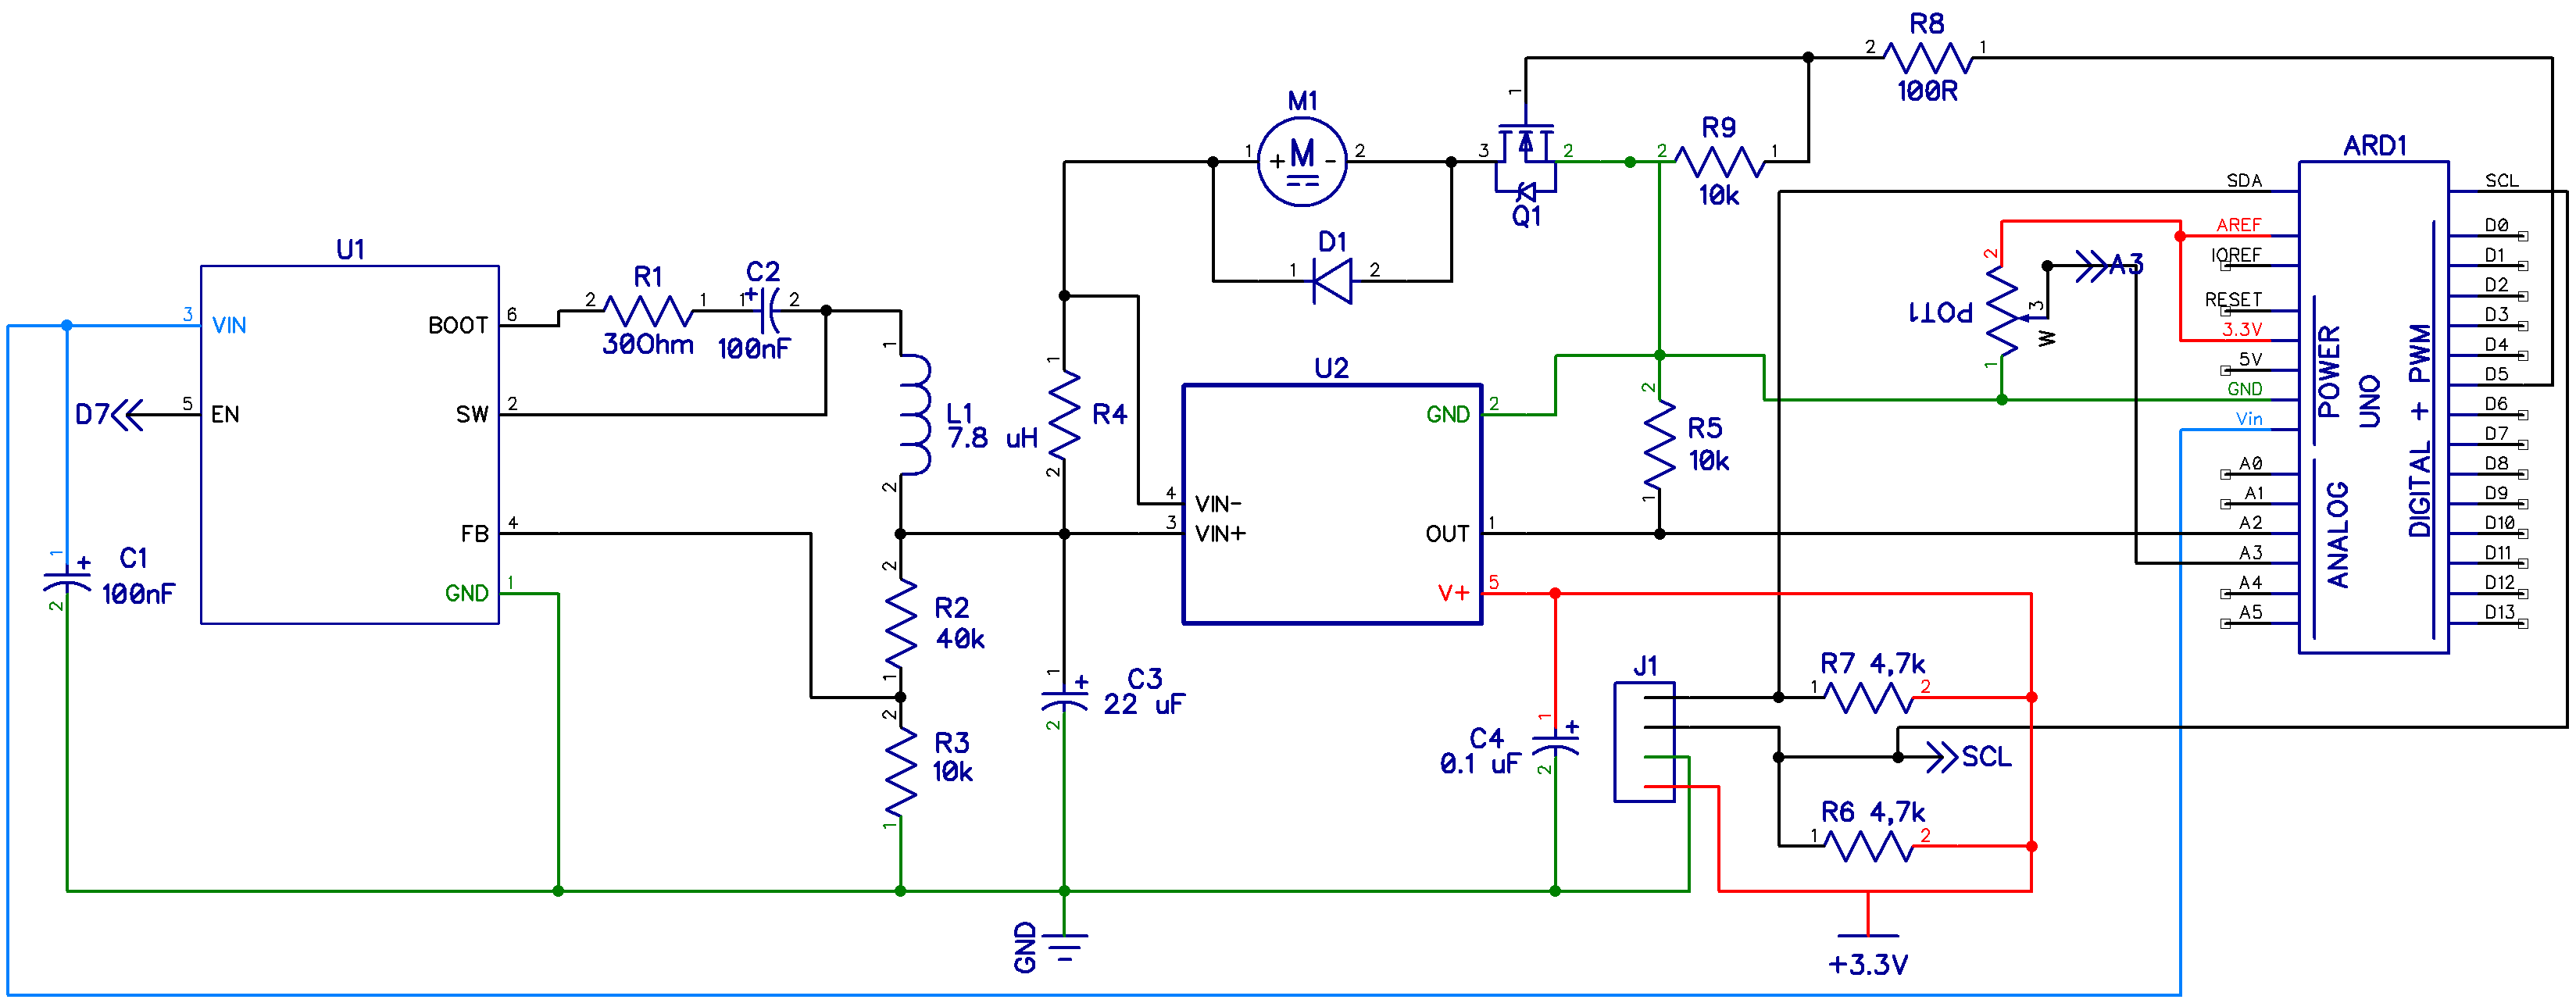
\includegraphics[width=\textwidth]{obr/TretiaSchema.png}
	\caption{Schéma zapojenia tretej verzie AeroShieldu.}\label{OBRAZOK 2.9}
\end{figure}